\documentclass{article}
\usepackage[utf8]{inputenc}
\newcommand{\ii}{{\bf i}}
\newcommand{\jj}{{\bf j}}
\newcommand{\kk}{{\bf k}}
\newcommand{\id}{{\bf 1}}
\newcommand{\hur}{\frac{\id+\ii+\jj+\kk}{2}}%The "Hurwitz point"
\newcommand{\hurwitz}{\Z\left[\hur,\ii,\jj,\kk\right]}%The set of Hurwitz integers
\usepackage{wrapfig}
\usepackage{calligra}
\usepackage[utf8]{inputenc}
\usepackage[dvips]{graphicx}
\usepackage{a4wide}
\usepackage{amsmath}
\usepackage{mathtools}
\usepackage{euscript}
\usepackage{amssymb}
\usepackage{amsthm}
\usepackage{amsopn}
\usepackage[colorinlistoftodos]{todonotes}
\usepackage{graphicx}
\usepackage[T1]{fontenc}
\newcommand\mybar{\kern1pt\rule[-\dp\strutbox]{.8pt}{\baselineskip}\kern1pt}

\usepackage{ulem}
\usepackage{xcolor}
\newcommand{\cs}[1]{\color{blue}{#1}\normalcolor}

%Matrix commands
\newcommand{\ba}{\begin{array}}
\newcommand{\ea}{\end{array}}
\newcommand{\bmat}{\left[\begin{array}}
\newcommand{\emat}{\end{array}\right]}
\newcommand{\bdet}{\left|\begin{array}}
\newcommand{\edet}{\end{array}\right|}
\newcommand{\inv}[1]{#1^{-1}}

%Environment commands
\newcommand{\be}{\begin{enumerate}}
\newcommand{\ee}{\end{enumerate}}
\newcommand{\bi}{\begin{itemize}}
\newcommand{\ei}{\end{itemize}}
\newcommand{\bt}{\begin{thm}}
\newcommand{\et}{\end{thm}}
\newcommand{\bp}{\begin{proof}}
\newcommand{\ep}{\end{proof}}
\newcommand{\bprop}{\begin{prop}}
\newcommand{\eprop}{\end{prop}}
\newcommand{\bl}{\begin{lemma}}
\newcommand{\el}{\end{lemma}}
\newcommand{\bc}{\begin{cor}}
\newcommand{\ec}{\end{cor}}
\newcommand{\lcm}{\mbox{lcm}}
\newcommand{\defn}{\fbox{definition}}
\newcommand{\prop}{\fbox{proposition}}
\newcommand{\stab}{\mbox{stab}}
\newcommand{\Aut}{\mbox{Aut}}
\newcommand{\orb}{\mbox{orb}}

\newcommand{\norm}{\righttriangle}

\newcommand{\and}{\wedge}
\newcommand{\or}{\vee}

%sets of numbers
\newcommand{\N}{\mathbb{N}}
\newcommand{\Z}{\mathbb{Z}}
\newcommand{\Q}{\mathbb{Q}}
\newcommand{\R}{\mathbb{R}}

\newcommand{\topT}{\mathcal{T}}
\newcommand{\standtop}{\mathcal{T}_{STD}}
\newcommand{\cc}{\mathcal{C}}


\documentclass{article}
\usepackage[utf8]{inputenc}
\newcommand{\ii}{{\bf i}}
\newcommand{\jj}{{\bf j}}
\newcommand{\kk}{{\bf k}}
\newcommand{\id}{{\bf 1}}
\newcommand{\hur}{\frac{\id+\ii+\jj+\kk}{2}}%The "Hurwitz point"
\newcommand{\hurwitz}{\Z\left[\hur,\ii,\jj,\kk\right]}%The set of Hurwitz integers
\usepackage{wrapfig}
\usepackage{calligra}
\usepackage[utf8]{inputenc}
\usepackage[dvips]{graphicx}
\usepackage{a4wide}
\usepackage{amsmath}
\usepackage{euscript}
\usepackage{amssymb}
\usepackage{amsthm}
\usepackage{amsopn}
\usepackage[colorinlistoftodos]{todonotes}
\usepackage{graphicx}
\usepackage[T1]{fontenc}
\newcommand\mybar{\kern1pt\rule[-\dp\strutbox]{.8pt}{\baselineskip}\kern1pt}

\usepackage{ulem}
\usepackage{xcolor}
\newcommand{\cs}[1]{\color{blue}{#1}\normalcolor}

%Matrix commands
\newcommand{\ba}{\begin{array}}
\newcommand{\ea}{\end{array}}
\newcommand{\bmat}{\left[\begin{array}}
\newcommand{\emat}{\end{array}\right]}
\newcommand{\bdet}{\left|\begin{array}}
\newcommand{\edet}{\end{array}\right|}
\newcommand{\inv}[1]{#1^{-1}}

%Environment commands
\newcommand{\be}{\begin{enumerate}}
\newcommand{\ee}{\end{enumerate}}
\newcommand{\bi}{\begin{itemize}}
\newcommand{\ei}{\end{itemize}}
\newcommand{\bt}{\begin{thm}}
\newcommand{\et}{\end{thm}}
\newcommand{\bp}{\begin{proof}}
\newcommand{\ep}{\end{proof}}
\newcommand{\bprop}{\begin{prop}}
\newcommand{\eprop}{\end{prop}}
\newcommand{\bl}{\begin{lemma}}
\newcommand{\el}{\end{lemma}}
\newcommand{\bc}{\begin{cor}}
\newcommand{\ec}{\end{cor}}
\newcommand{\lcm}{\mbox{lcm}}
\newcommand{\defn}{\fbox{definition}}
\newcommand{\prop}{\fbox{proposition}}
\newcommand{\stab}{\mbox{stab}}
\newcommand{\Aut}{\mbox{Aut}}
\newcommand{\orb}{\mbox{orb}}

\newcommand{\norm}{\righttriangle}

\newcommand{\and}{\wedge}
\newcommand{\or}{\vee}



%sets of numbers
\newcommand{\N}{\mathbb{N}}
\newcommand{\Z}{\mathbb{Z}}
\newcommand{\Q}{\mathbb{Q}}
\newcommand{\R}{\mathbb{R}}
\newcommand{\TT}{\mathbb{T}^2}
\newcommand{\RPT}{\mathbb{RP}^2}
\newcommand{\ST}{\mathbb{S}^2}

\newcommand{\topT}{\mathcal{T}}
\newcommand{\standtop}{\mathcal{T}_{STD}}
\newcommand{\cc}{\mathcal{C}}


\title{Topology}
\author{August bergquist}


\begin{document}

\maketitle
\fbox{Theorem} If $M = \Big{\#}_{i  =1}^n M_i$, then $M$ is orientable if and only if $M_i$ is orientable for all $1\le i\le n$. \\

Throughout our work, it has not been the most trivial of tasks in determining the fixing numbers of graphs, particularly for $K_{n}$ graphs, since we would have to exhaust all of the automorphism groups of a given $K_{n}$ graph. FIGURE \ref{CompleteGraphs} and Table ~\ref{tab:template} demonstrates some of our results we have done for $K_{6}$, the complete graph with $6$ vertices. 


\fbox{proof} We will begin by showing that if $M$ is orientable, then all $M_i$ that make up $M$ as a connect sum are also orientable. Suppose by way of the contrapositive that some $M_i$ is not orientable. Then $M_i$ contains a Mobius strip, as follows from Theorem 11.40. Because $M_i$ contains a Mobius strip, we know that for any of its polygon representation, there are identified edges of the same orientation. Let $P$ be an arbitrary polygon representation of $M_i$. If we name this edge $a$, then $P$ can be represented by the word $aAaB$, where $A$ and $B$ simply denote the other edges of $P$ between $a$ and $a$. Concatenating with the other $M_j$s will not get rid of any of our edges, as shown in the picture below. Hence the concatenation of all of them, if put as a word for a polygon representation, will have the form $aAaBC$, where $C$ denotes a word for a polygon representation of the connected sum of all $M_j$s other than $M_i$. Since the connect sum of all of these is $M$ by definition, $M$ has a polygon representation that can be represented with the word $aAaBC$. Cutting along the edges labeled $a$ to create a boundary, we have a Mobius strip. Hence $M$ contains a Mobius strip, which by Theorem 11.40 means that $M$ is not orientable. See the figure for a visual explanation for what we are doing here.\\

\begin{figure}[htbp]
\centerline{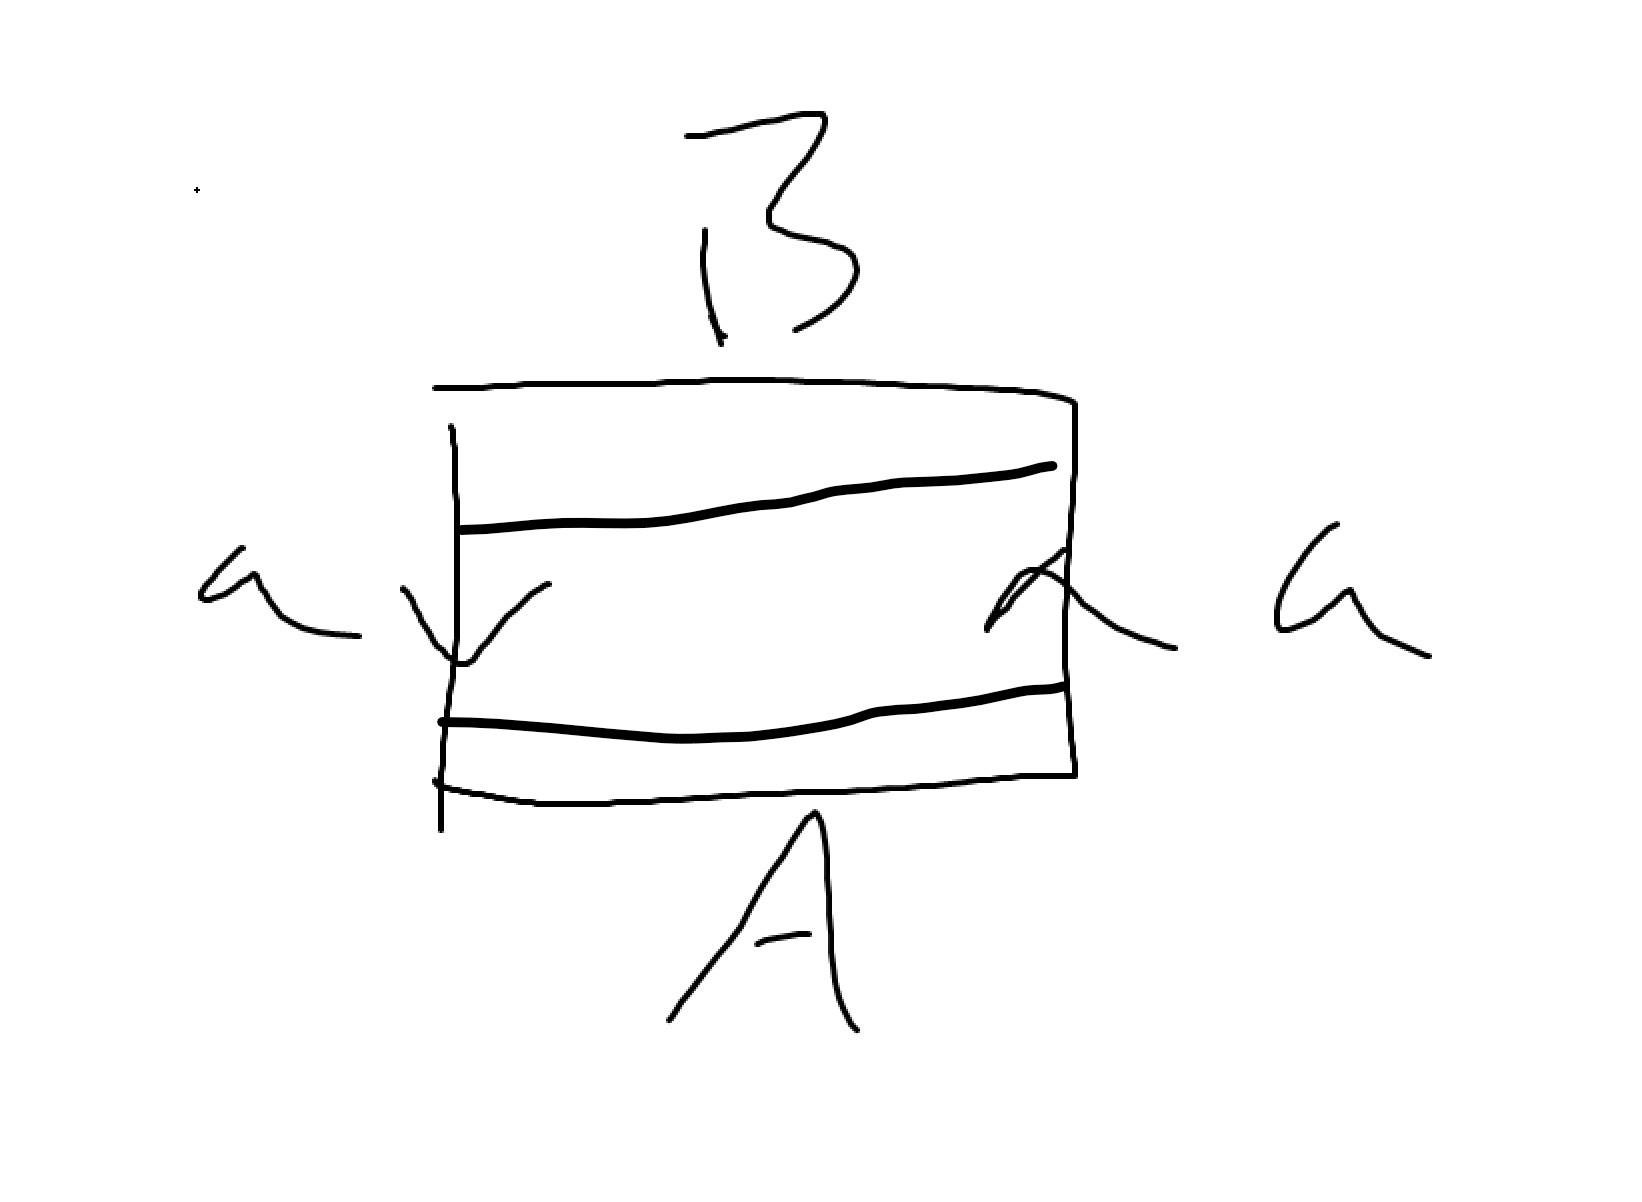
\includegraphics[scale=0.25]{homework/mobiusstrip.png}}
\caption{Polygon representation for $M_i$ with a Mobius strip}
\label{fig}
\end{figure}

\begin{figure}[htbp]
\centerline{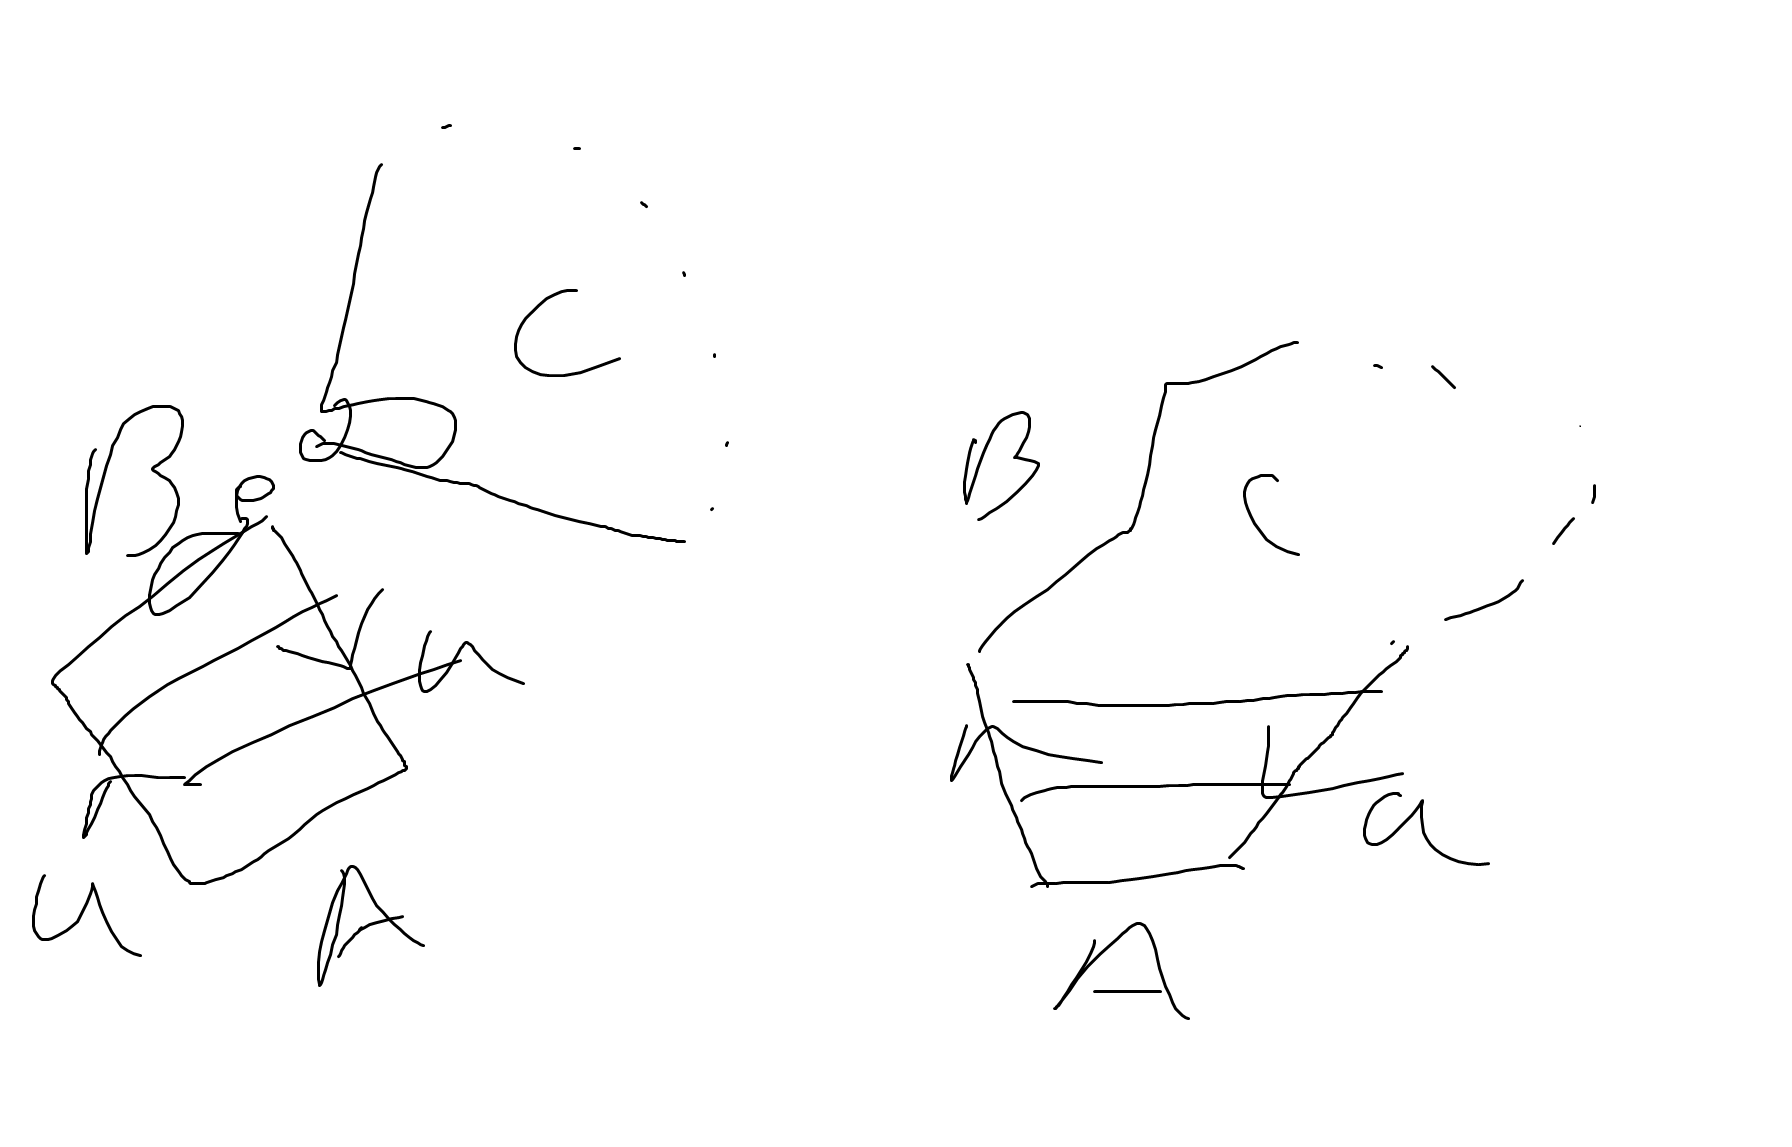
\includegraphics[scale=0.25]{homework/connect_sum.png}}
\caption{Visual representation of this proof. Notice how we can still find a Mobius strip using the edges $a$ (the other arrow edge on the second polygon should be labeled $a$). What we have done is tken a small disk out of the polygon representations, and identified the corresponding edges. Doing this does not get rid of edges $a$, nor does it change their orientations.}
\label{fig}
\end{figure}

Now to show that the converse is also true, suppose that each $M_i$ is orientable. By the Classification of $2$ manifolds, there are three options for each $M_i$: Either (1) $M_i = \Big{\#}_{j=1}^m \TT$, (2) $M_i = \Big{\#}_{j=1}^m \RPT$, or (3) $M_i = \ST$. Since $M_i$ is orientable, and since $\RPT$ is not, by the first part of this proof it follows that (2) cannot be the case, as this would be a contradiction. Hence the only two possibilities for each $M_i$ are for $M_i$ to be a connect sum of $m$ tori, or a sphere. Since connect summing a 2-manifold with a sphere does nothing to the original shape, there are two cases. Either all $M_i$ are spheres, or some of them are tori. If all $M_i$ are spheres, then $M$ is a sphere as well, which is orientable. Suppose then that some $M_i$ are tori. Since order doesn't matter in connect sums, we can move all of the spheres to the first part of the connect sum, combine them into one, and we have 
$M = \Big{\#}_{i=1}^nM_i = \ST \#_{i = 1}^n\TT$. Since each of the tori will have a polygon representation with a word $ab\inv{a}\inv{b}$, our connect sum will simply concatenate each of these words to get us $ab\inv{a}\inv{b}...cd\inv{c}\inv{d}$ as the word for our polygon representation of $M$. The only way get a Mobius strip is for the polygon representation to include a pair of edges with opposite orientations, which we do not. Hence $M$ is orientable, as follows from Theorem 11.40.
\end{document}